\documentclass[]{book}
\usepackage[paperwidth=6in, paperheight=9in]{geometry}
\usepackage[overload]{textcase}
\addtolength{\oddsidemargin}{0.375in}
\addtolength{\evensidemargin}{-0.375in}

\newcommand{\blankpage}[1]{
    \newpage
    \thispagestyle{#1}
    \mbox{}
    %\newpage
}
\usepackage{graphicx}

\usepackage{floatpag}
\floatpagestyle{empty}
\rotfloatpagestyle{empty}

\renewcommand{\chaptermark}[1]{\markboth{\slshape{#1}}{}}

\usepackage[nouppercase]{scrpage2}
\pagestyle{scrheadings}
\chead{\headmark}
\ihead[]{}

\usepackage{verse}

\newcommand{\makeTitlePages}[6]{
    \pagenumbering{gobble}
    \blankpage{empty}
    \blankpage{empty}
    \newpage
    \vspace*{\fill}
    {\centering\Huge\bf\centering #1
    \vspace*{\fill}

    \title{#1}
    \author{#3}
    \maketitle}

    \cleardoublepage
    \pagenumbering{roman}
    \setcounter{page}{7}
}

%% Patch for blank pages between chapters
%% which disables the current page style
\makeatletter
\def\cleardoublepage{\clearpage\if@twoside \ifodd\c@page\else
  \hbox{}\thispagestyle{empty}\newpage\if@twocolumn\hbox{}\newpage\fi\fi\fi}
\makeatother

\usepackage{multicol}
\usepackage{xcolor}
\usepackage{allrunes}
\usepackage{xstring}

\usepackage[nf]{coelacanth}
\usepackage[T1]{fontenc}
%% The font package uses mweights.sty which has som issues with the
%% \normalfont command. The following two lines fixes this issue.
\let\oldnormalfont\normalfont
\def\normalfont{\oldnormalfont\mdseries}

\noexpandarg\exploregroups
\newcommand\dwarvenSpace[1]{\StrSubstitute{#1}{ }{\textarm{.}}}
\newcommand\dwarvenFullStop[1]{\StrSubstitute{#1}{.}{\textarm{\tripleeye}}}
\newcommand\dwarvenA[1]{\StrSubstitute{#1}{a}{\textara{\oe}}}
\newcommand\dwarvenAA[1]{\StrSubstitute{#1}{\=a}{\textara{\oe}}}
\newcommand\dwarvenB[1]{\StrSubstitute{#1}{b}{\textarm{b}}}
\newcommand\dwarvenD[1]{\StrSubstitute{#1}{d}{\textarm{\o}}}
\newcommand\dwarvenG[1]{\StrSubstitute{#1}{g}{\textarc{\RR}}}
\newcommand\dwarvenH[1]{\StrSubstitute{#1}{h}{\textara{h}}}
\newcommand\dwarvenI[1]{\StrSubstitute{#1}{i}{\textara{\j}}}
\newcommand\dwarvenII[1]{\StrSubstitute{#1}{\=\i}{\textara{\j}}}
\newcommand\dwarvenK[1]{\StrSubstitute{#1}{k}{\textarc{g}}}
\newcommand\dwarvenL[1]{\StrSubstitute{#1}{l}{\textarm{y}}}
\newcommand\dwarvenM[1]{\StrSubstitute{#1}{m}{\textara{m}}}
\newcommand\dwarvenN[1]{\StrSubstitute{#1}{n}{\textara{d}}}
\newcommand\dwarvenO[1]{\StrSubstitute{#1}{o}{\textarc{\ng}}}
\newcommand\dwarvenTH[1]{\StrSubstitute{#1}{th}{\textarm{\th}}}
\newcommand\dwarvenR[1]{\StrSubstitute{#1}{r}{\textarm{m}}}
\newcommand\dwarvenS[1]{\StrSubstitute{#1}{s}{\textarm{s}}}
\newcommand\dwarvenT[1]{\StrSubstitute{#1}{t}{\textarm{\ae}}}
\newcommand\dwarvenU[1]{\StrSubstitute{#1}{u}{\textara{\ng}}}
\newcommand\dwarvenUU[1]{\StrSubstitute{#1}{\=u}{\textara{\ng}}}
\newcommand\dwarvenV[1]{\StrSubstitute{#1}{v}{\textarm{\r}}}
\newcommand\dwarvenZ[1]{\StrSubstitute{#1}{z}{\textarm{x}}}
\newcommand\dwarven[1]{%
	\large{%
	\lowercase{%
	\dwarvenFullStop{%
	\dwarvenSpace{%
	\dwarvenTH{%
	\dwarvenAA{\dwarvenA{%
	\dwarvenB{%
	\dwarvenD{%
	\dwarvenG{%
	\dwarvenH{%
	\dwarvenII{\dwarvenI{%
	\dwarvenK{%
	\dwarvenL{%
	\dwarvenM{%
	\dwarvenN{%
	\dwarvenO{%
	\dwarvenR{%
	\dwarvenS{%
	\dwarvenT{%
	\dwarvenUU{\dwarvenU{%
	\dwarvenV{%
	\dwarvenZ{%
		#1%
	}}}}}}}}}}}}}}}}}}}}}}}}}
	\normalsize
}

\newcommand{\dwarvenDef}[3]{%
	\item[#1] \emph{\color{gray}#2.} #3
%
	%\dwarven{#1}
}
\newcommand{\dwarvenDefOld}[3]{%
% 1 word
% 2 word type
% 3 definition
	%\item[#1] \dwarven{#1}
	\item[#1] \dwarven{#1}

\emph{\color{gray}#2}. #3
}

\newcommand{\dwarvenInscription}[1]{

\vspace{1em}
	\noindent
	\begin{center}
	{
		%\large
		\dwarven{#1}
	}
	\end{center}
\vspace{1em}

}

\newcommand{\divider}{
\vspace{1em}

\hfill
%\rule{3in}{0.5pt}
***
\hfill{}

\vspace{1em}
}

\makeatletter
\def\cleardoublepage{\clearpage\if@twoside \ifodd\c@page\else
  \hbox{}\thispagestyle{empty}\newpage\if@twocolumn\hbox{}\newpage\fi\fi\fi}
\makeatother

\usepackage{floatpag}
\floatpagestyle{empty}
\rotfloatpagestyle{empty}

\renewcommand{\chaptermark}[1]{\markboth{\slshape{#1}}{}}

\usepackage[nouppercase]{scrpage2}
\pagestyle{scrheadings}
\chead{\headmark}
\ihead[]{}

\usepackage{tocloft} % the tocloft package lets you redefine the Table of Contents (ToC)
\renewcommand\cftchappresnum{Chapter } % prefix "Chapter " to chapter number in ToC
\renewcommand\cftchapdotsep{\cftdotsep}
\renewcommand\cftchapnumwidth{5em}


\newcommand{\poem}[1]{%
	\addcontentsline{lot}{table}{#1}
}
\renewcommand{\listtablename}{List of Songs and Poems}


\begin{document}
\frontmatter
%\makeTitlePages{The Dwarf and the Sword of Purity}{}{Timothy Gurto}{2021}{}{}

%\newpage
%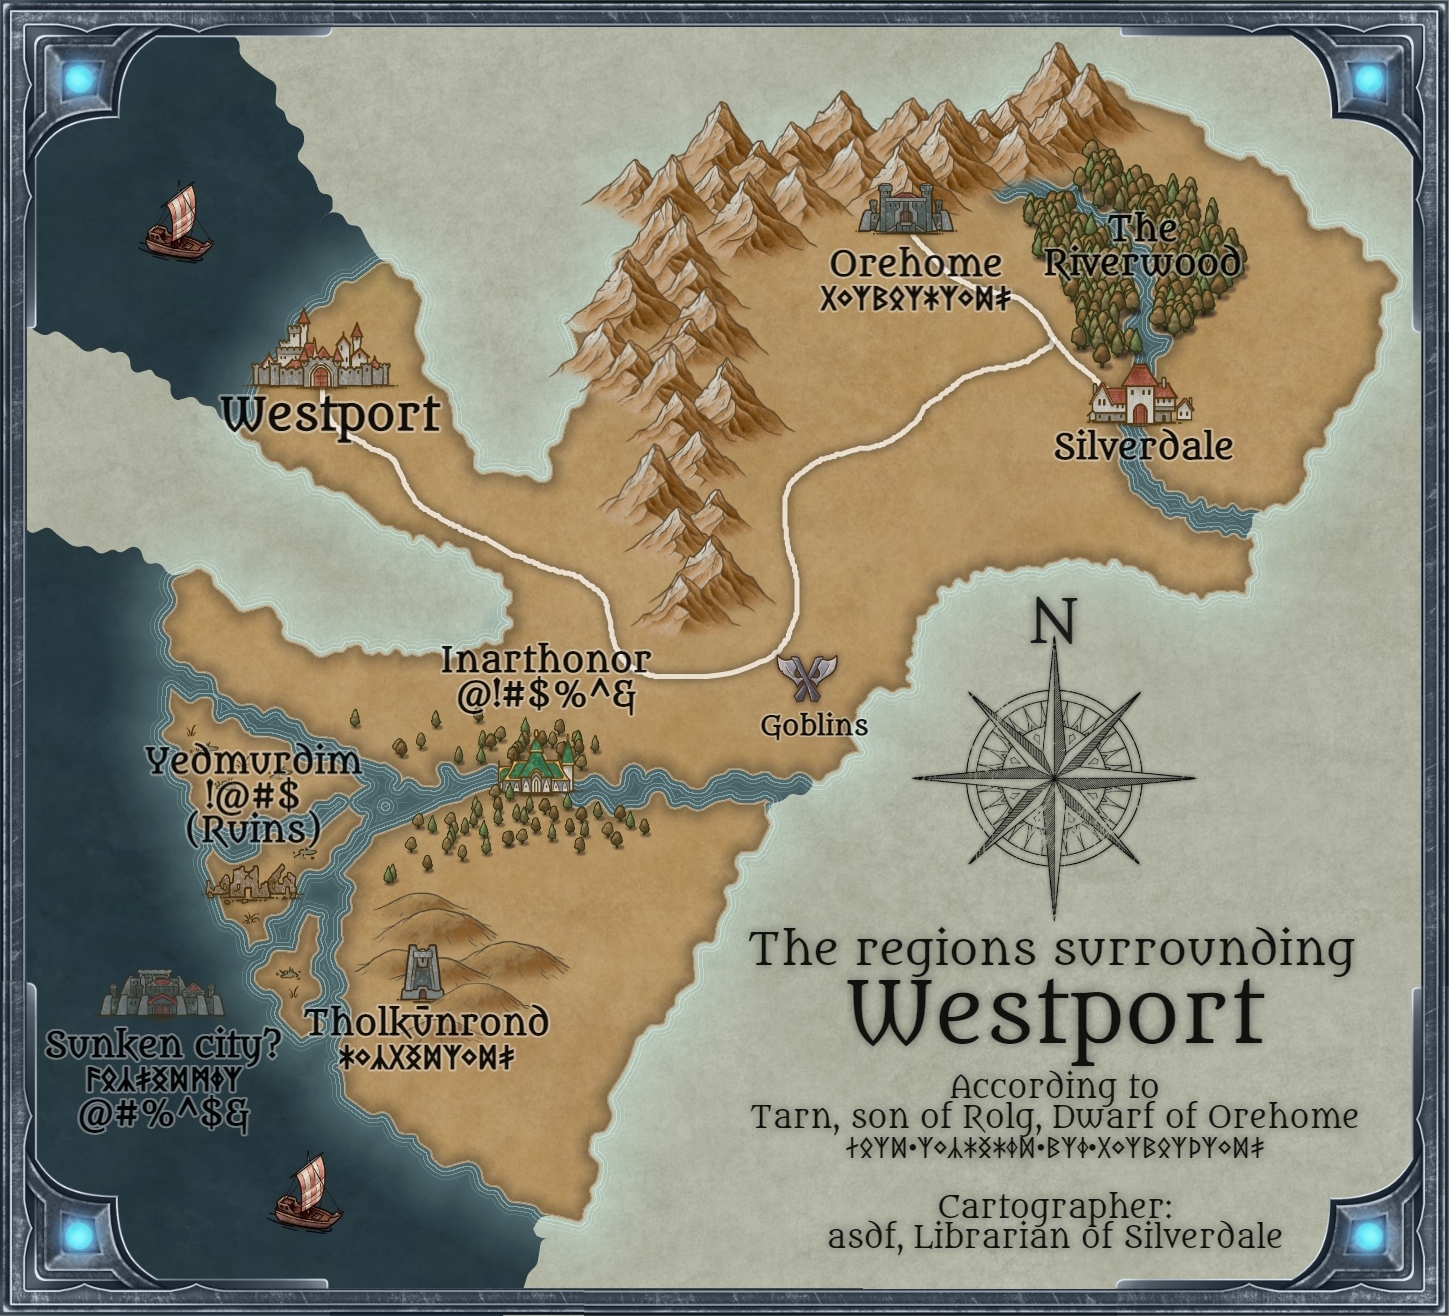
\includegraphics[trim=0 0 19cm 0, clip, width=\textwidth]{map}
%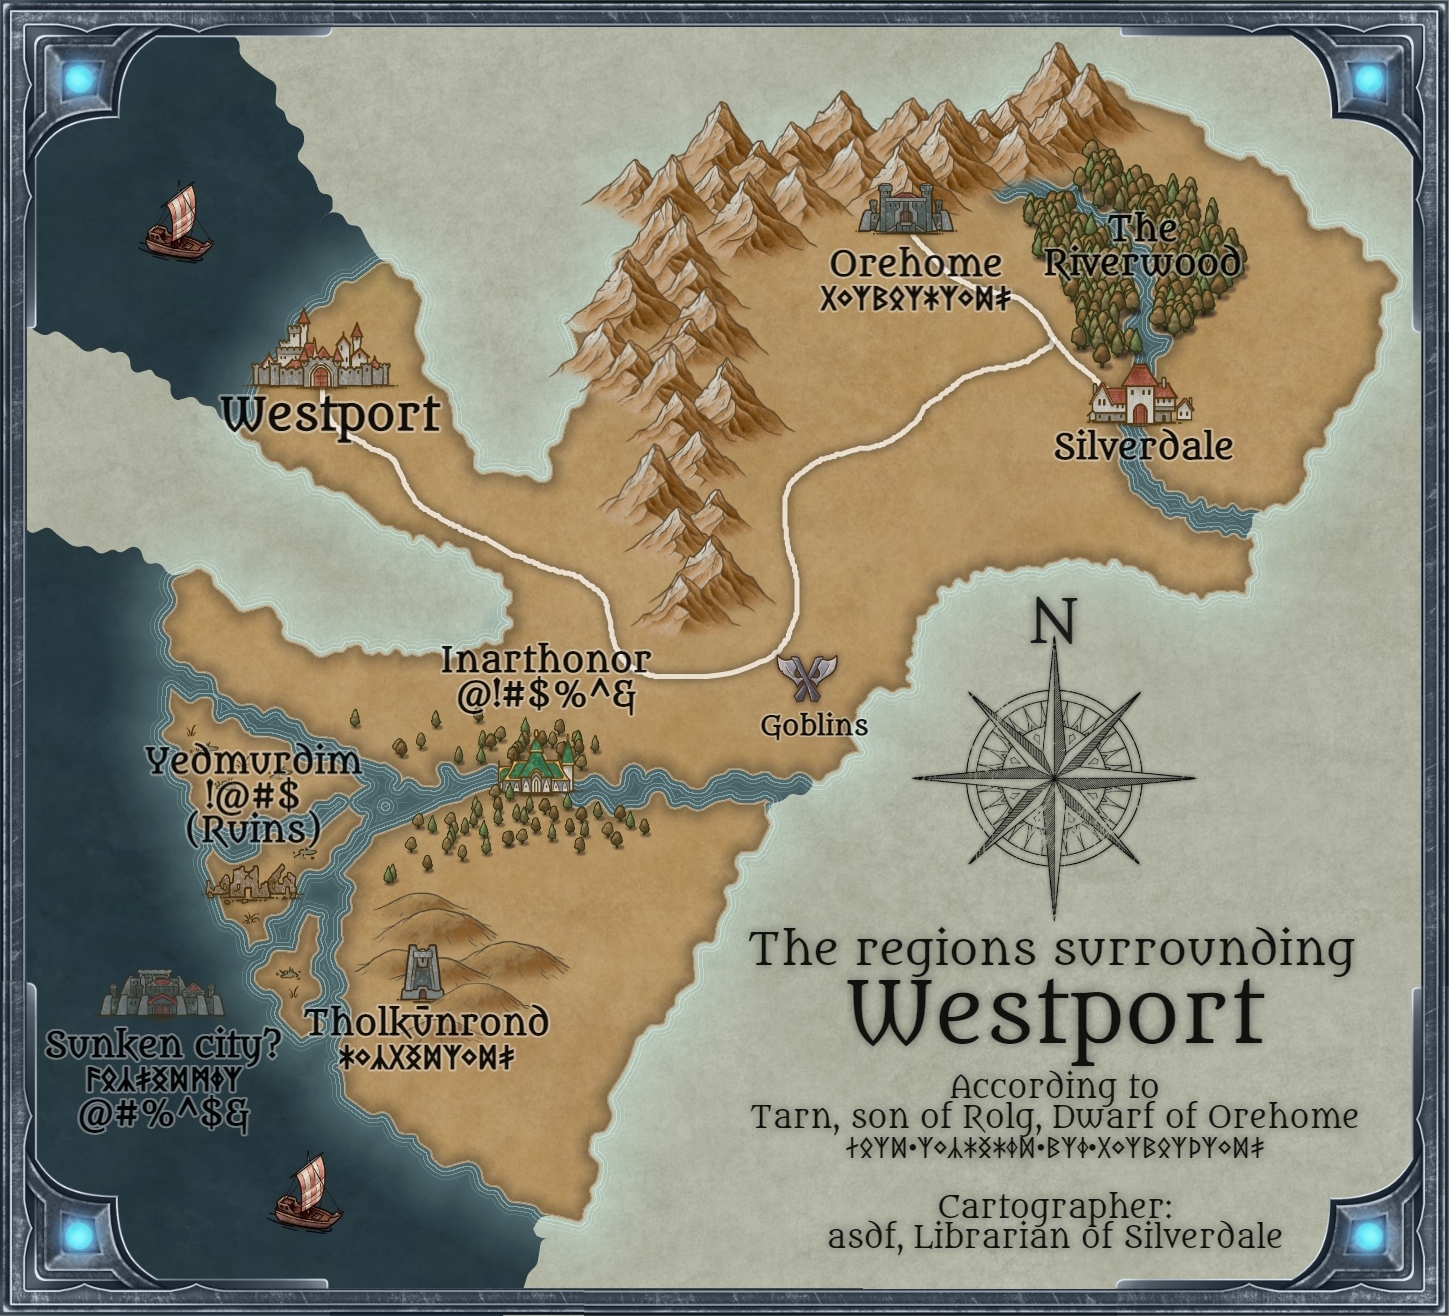
\includegraphics[trim=19cm 0 0 0, clip, width=\textwidth]{map}

\cleardoublepage
%\tableofcontents % commented out because the dots dirty the word count

%\addcontentsline{toc}{chapter}{List of Songs and Poems}
%\listoftables

\mainmatter
\chapter{Ripples in the Stone}
Tarn, son of Rolg, stood straight and still, his eyes peering over the city's entrance hall one last time before he ended his shift.  Guarding the city was as uneventful today as it usually was; the worst invaders Tarn had ever needed to repel from the city were bears and other wild animals.  In a more turbulent time he may have stood against an attacking horde, or have been part of an army marching off to fight for some great cause, but in this age of peace he stood \emph{inside} the gates, looking inwards.  Not that he minded---he was a dwarf, after all, and like most of his kind he was most comfortable nestled within the carved bosom of his mountain.

The entrance hall was cavernous and showy.  Wide columns stretched to the ceiling, so high that it was hard to see their tops among the distant dark.  The floor of the hall was tiled with polished marble, tapping sharply with each footstep from the dwarves going about their business.  Because it was so close to the main gate, over the generations this hall had developed into a marketplace for dealing with visitors from outside.  The city received only one or two traders per day, and so most of the merchants here still served the local dwarves.  Occupying the stall nearest to Tarn was a silversmith, whose tables were decorated with scales and stacks of coins and ingots.  Silver was the city's main export, and it was mined and smelted here in the mountain.  In the stall next to that one was a wood carver, selling ornaments.  There were larger markets deeper within the city, but this was the place to find those goods made to appeal to outside buyers.

The stone walls were engraved with elaborate patterns and images.  These walls were carved in-situ, straight into the original rock, and not placed there.  Marbled throughout them were veins of a pale blue mineral which the dwarves named simply Omunkorb, or ``Blue-ore'' in the language of Men.  Where the blue touched the engravings, it was polished to be bright and clear, so as to be more easily seen.  Omunkorb permeated much of the city, and the dwarves generally kept it intact wherever found: they could find no functional use for it, only decorative, and it had become a source of pride for them.  Thus was the city itself called \korbarthrond---``Orehome''.

A large inscription was engraved prominently on one of the high walls flanking the entrance hall, a message to citizens and visitors alike.  Its glyphs consisted of the hard, straight marks of the Dwarven script, adapted to be carved into hard materials.  The inscription read:
\dwarvenInscription{%
bamk azthu thaku trobu gi brolzolg\\%
dult korb krithsulb gorg izun gi kugzolg.}
Roughly translated, it means:
\settowidth{\versewidth}{Like ore, innate and polished in our walls,}
\begin{verse}[\versewidth]\poem{The exhortation of \korbarthrond}
Like ore, innate and polished in our walls,\\
should you be true yet shine within these halls.
\end{verse}

Tarn always enjoyed patrolling here, because it gave him an opportunity to admire the craftsmanship of those wall engravings.  The images depicted various stories from the history and myth of the city and her people, and they exhibited the care and love of fine work that most dwarves applied to their various vocations.  Guardwork afforded little opportunity for Tarn himself to scratch this itch, and so he instead found opportunities to appreciate the work of others.

His replacement arrived just as the deep bell announced shift's end.

``All quiet today,'' said Tarn.

The other guard smiled and nodded, and Tarn began to head home, while the others in the market area mostly stayed put.  Craftsmen and merchants worked on their own time; it was only the city workers like Tarn who followed the shift system.  He walked home faster than usual, as he had arranged to meet a long-time friend of his after work today: Lawrence, a human trader who was visiting the city.

Following a number of corridors and common areas, Tarn reached his quarters, a modest apartment carved into the mountain.
Tarn's admiration for fine work extended beyond enjoying the city's commons, and into into his home.  He maintained a collection of personal treasures: gold rings embedded with brightly coloured gemstones, and small figures of polished silver and carved stone.  Taking pride of place on a shelf near his bed was a scale model of the mountain, about the size of his fist and carved from a solid piece of Omunkorb.

The bulk of Tarn's wealth lay in a cache of ingots and coins made from gold and silver, which he loved for their precision, detail and shine almost as much as for their value.  The silver was mined here in \korbarthrond, but the gold needed to be imported as the mountain had none beneath it.  Most of the coins were struck here though, as \korbarthrond, like most every other dwarven city, took advantage of every opportunity to make its mark.  That being said, Tarn did have a few gold coins from other cities, as they sparked a romantic fantasy of the wider world, and of dwarves spread far abroad yet engaging in the same pursuits and industries that they enjoyed here.  While Tarn had no interest in actually \emph{seeing} those far-off cities, he felt reassured---and proud---to be a part of something larger.

Tarn changed out of his uniform, and headed to the tavern nearest his apartment.  He found Lawrence already there, at a table with two mugs of beer in front of him.  As with all men, Lawrence was tall and lanky compared with most dwarves, with a small nose and shallow eyes.  Seeing Tarn, he stood up with his arms outstretched.

``Tarn, my old friend!  How are you?''

``Good, good.  And you?  How was the road?'' Tarn replied, sitting.

Lawrence lived in Silverdale, the town of men in the valley below the mountain and the closest major settlement.  Silverdale was built on the \korbarthrond\ River, which flowed east from the mountain towards the sea.  Lawrence didn't sail up the river, though: although it was wide, it meandered through a thick, treacherous forest---called Riverwood by the men---that had claimed many ships.  And so, while they could engage in water trade downstream, no trader came to \korbarthrond\ except by road and through the main gate.

``The days were quiet and the nights were mild.  All a man can ask for,'' he replied.


Tarn leaned forward.  ``Anything new in town?  What are the men up to these days?''  Humans were always coming up with new designs, theories, and technologies.  Many were amusing failures, but sometimes real innovations took place.  On his last visit, Lawrence had told him about an alchemist who had accidentally created a new kind of medicine!

``Nothing much in Silverdale, but I did hear that Westport is experimenting with new kinds of fertiliser.  If it works, they think they can improve crop yields by a lot.''  Westport was a major human city, the most influential power in the region.

The two old friends continued talking about their respective cities and peoples, and exchanging jokes and stories, and they soon finished their drinks.

Tarn put his empty mug down and wiped his beard with the back of his hand.  Lawrence had no beard at all to match his dark-red hair, though Tarn understood facial hair to be less common among men, and a matter of personal style.  Dwarves, on the other hand, grew their beards long by convention, braiding and decorating them with care.  Seeing anyone clean shaven, even a man, and even a familiar man like Lawrence, still felt odd even after many years of friendship.

``Can I buy you another?'' Tarn asked.  Then, jokingly, ``or would you prefer water instead of beer?''

``Just because I don't bathe in the stuff like a dwarf, doesn't mean I can't hold my own!''

Dwarves drank beer almost as much as they did water, and on social occasions like this there was no excuse to drink anything else.

``Anyway, I already tried ordering some,'' Lawrence continued.  ``The bartender said they were out.''

``Out of water?''

``And not just today.  He said they'd been having trouble for days.''

``Odd,'' said Tarn, trying to remember the last time he'd replenished his own water barrel.

The city had one primary well near the centre, going deep into the aquifer.  Other, smaller wells were connected to it.  Tarn had never known any of the wells to go dry.

Lawrence went on.  ``In fact, that's exactly what brings me to the city this time.  Your king ordered a shipment of water from the river, and I just carted in eight full barrels of it.''

If there was a problem with the city's water supply, Tarn wanted to know about it.  He may not have been able to do much about that sort of problem, but he felt some level of responsibility over the city---perhaps an inclination that came with his position as a guard---and wanted to keep on top of issues like this.  So he resolved to get some answers.

After another round of beer, Tarn and Lawrence said their goodbyes. Lawrence headed to the inn and stables near the front gate, where he had a room rented and his cart was interred.  Tarn headed towards the heart of the mountain, to visit the king and ask him what was going on.

%\chapter{The King's Request}

Two uniformed guards stood in front of the throne room.  It was blocked by a large door of dark wood, banded at the top and bottom with iron engraved in a complex geometric pattern.  In the middle of the door was an outline of their mountain, carved into the wood and inlaid with bright silver wire.  The guards smiled as they recognised their peer.

``Guardsman Tarn!  What brings you to the throne room?''

``Hello boys.  I'd like an audience with His Majesty.''

One of the guards muttered something through the door to someone on the other side, and received a low, muffled response.  He told Tarn to wait for a moment.  The three guards chatted for a few minutes, until eventually the low voice spoke again from the other side of the door.

``You can go ahead in, Tarn,'' said the guard.  He pulled the handle and the door swung open.

Athzad, son of Valkold, was the king of \korbarthrond.  He had reigned for nearly twenty years, and was well-regarded by the citizens of the mountain.  King Athzad had a long, thick, brown beard, split into three with silver thread braided into each part.  He wore a crown on his head, a band of patterned gold decorated with many jewels, uniquely coloured but all cut to the same size and shape, brightly reflecting the flickering light from the throne room's torches.  The throne beneath him was solid stone, carved in precise straight angles and rippled with polished Omunkorb.

Tarn entered the room, approached the throne, and bowed.  The guard standing next to the throne stared straight ahead.

``What can I do for you, guardsman?'' King Athzad asked.

``Your Majesty, I have heard that the city is having trouble with its water supply.  I want to know if it's true, and if possible, the cause.''

The king sighed.  ``You heard correct, though this is not publicly known, and I ask you not to spread it around and cause a panic.

``For about two weeks now, dwarves have been getting sick from our wells.  Something goes wrong in the gut.  We don't know what's causing it.''

``So that's why we're importing water?''

``That's right,'' the king answered.  ``The only water provided for drinking is what we can get from outside.  The wells are restricted to industrial uses, washing and brewing.''

``Brewing?  Is our beer being poisoned?'' Tarn snapped quickly, in a tone not fit for the throne room.  The guard by the throne raised an eyebrow and tightened his grip on his spear.

The king maintained his steady voice.  ``I understand your concern.  Boiling the water appears to make it safe, and so our beer is not dangerous due to the way it's made.''

Tarn took a deep breath.  ``I apologise, Your Majesty.  Is there anything we can do about it?'' he asked.

``We are pursuing a number of strategies,'' came the reply.  ``One team is exploring the darker caves and tunnels for potential new sources.  Another is engaged in fetching water from the river outside.  And we will continue importing what we need until a solution is found.''

Tarn was not optimistic.  Water sources within a mountain are rare; and anything truly accessible would have been found by now.  Fetching water from the river, through that forest, was too labour-intensive.  And long-term, buying water seemed like economic suicide.  But he held his tongue, and took care to get his thoughts in order before speaking.  He thought about Lawrence's stories about men, and their experiments and advances.

``Your majesty,'' he began slowly, ``I think it's worth sending somebody to the human town downriver, to see if they know of a solution.''  Tarn was careful not to directly criticise the king's other strategies, or to suggest that Men had any kind of superiority over Dwarves.
``Men lack our sense of beauty and accomplishment, and for want of a similar greatness they constantly try new things and push new boundaries with plants and animals and machinery.  They may have a technology or a medicine that we do not.''

King Athzad considered this silently for a moment, before responding, ``Very well.  If you believe the men of Silverdale possess some secret that will save \korbarthrond, then you will be the one to go there, and determine for yourself whether they have anything useful''.

``Me?'' asked Tarn, blinking.

``With your affinity for the men, you are the best placed to find the ways in which they can help us,'' replied the king with an almost imperceptible hint of sarcasm.

The decision had been made.  Tarn thanked the king, bowed, and took his leave.

Tarn walked slowly back towards his quarters, trying to comprehend what had just happened.  He'd been asked by the king to go on a journey: days of road travel, to a Human town.  Tarn had never strayed far from the mountain, and had slept every night of his life within Korbarthrond.  He shuddered.

Could he abandon his guard responsibilties to go on this mission?  There was a sense of duty drilled into him through years of training and following orders.  But this was an order from King Athzad himself!  Surely he was just making excuses at this point.  Finding himself suddenly desiring counsel, he turned and, instead of going home, decided to visit a close friend.  Tarn followed the corridor until he came to the door with the desired inscription:

\dwarvenInscription{orvi kogugim}

\emph{Orvi, son of Kog}.  A metalworker, Orvi had been Tarn's friend since childhood.  Tarn knocked on the door.  About a minute later, the door opened.

``Tarn?''  Orvi rubbed his eyes.  He was wearing his dressing gown and holding a lantern.

``Hello my friend.  I'm sorry for calling so late, but something's troubling me.''

``Of course, come in!''  Orvi stepped aside, allowing Tarn to enter the apartment.  He turned up the lantern and hung it on the wall to illuminate the sitting room.

Like Tarn's, Orvi's home was decorated with a number of crafted goods, but here most of them had been made by Orvi himself.  Hanging on the far wall was a large knife, its shiny steel blade etched with words---probably merely ceremonial or decorative; it didn't look to Tarn like it had ever been used.  On Orvi's table were a fruitbowl and water jug, made from bronze with elaborate patterns engraved on them and delicate moulded shapes dancing around the rims.   Sitting on a shelf above the fireplace was a row of small ingots, perfectly shaped and polished to a mirror finish, each of a different metal.  Other shelves and furniture proudly displayed various machinery, figures, and coins, all metal and all beautiful.  Upon seeing these fine creations---and, almost as a reflex, thinking about the work and care that went into them---Tarn quickly calmed down, feeling at peace.

He sat at the table, and looked first at the water jug and then at Orvi.  ``There's a problem with the city's water supply.''  After reflecting for a moment, Tarn added, ''the king asked me not to spread it widely and create a panic, so please keep this to yourself.''

Orvi nodded.  ``What kind of problem? I went down to the well just this morning.  I use water every day to quench my pieces of work, and I haven't noticed any issues.''

``The wells are still operating, and open for industrial uses.  We just can't use them to get drinking water.  Some sort of poison, apparently."  Tarn sighed.  ``I disagreed with the king's planned course of action, and in exchange he strongarmed me into journeying to Silverdale.''

``What \emph{was} the king's planned course, that you found it so disagreeable?'' Orvi asked.

``One team is searching the mines for new wells or underground streams.  Another is starting to haul water in from the river.  The city is also buying water from Silverdale---my friend Lawrence brought some in just this week.''

``And you don't think those will work?''

``Not in the long term, no,'' Tarn answered.  ''I think the search will fail, and the other two approaches are too expensive or impractical.''

Orvi nodded slowly.  The silence made Tarn feel uncomfortable; defensive.  ``You disagree?''

``I think they're worth trying.  After all, we need to do something.  What are you supposed to do in Silverdale?"

``The king wants me to ask around, and see if I can find any advanced technology or medicine that can help us.  It was my suggestion, actually; all he did was volunteer me for the job.''

Orvi knew how close Tarn was with his Human friend Lawrence, and that he had a soft spot for Men in general.  ``You seem optimistic about it.''

``Less pessimistic than about the other ideas, I suppose.  But I still feel uncomfortable about the whole thing."

``About your chances?''

``No,'' Tarn answered, ``about leaving for Silverdale.''

``Ahh,'' sighed Orvi sympathetically.  ``It's natural to want to stay here, underground; straying outside is asking for trouble.  So don't discount your gut feeling about this journey.''

``But don't you think it's worth trying, even if I \emph{am} scared, for the sake of the city?''

Orvi thought for a moment, and then spoke slowly, deliberately.  ``If you want my honest answer, I think you're being too idealistic about the Men.  They don't have the answer for everything.  I don't think you're going to find much out there.  And in the mean time, it sounds like the king has things under control.''

His friend's confidence gave Tarn some relief.  He thanked Orvi for his time, wished him well, and left.  It had been a long evening of merry reunions and sobering discussion, and eventually Tarn managed to get to sleep.

The next day Tarn was again on duty, posted at one of the city's banks.  At least by working he was able to contribute---who knows how much time he could have wasted by travelling, and with the possibility of no benefit!

But it was hard to focus on his work.  The water problem still gnawed at him, pulling at his attention constantly.  \emph{How long can the city survive without drinking water?  How long could the citizens live off only beer, wine, and whatever dribbles of water could be imported?  How long could the economy bear those endless imports?}  There was no guarantee that a new water source could be found.  And if one was, who was to say that it wouldn't share the same taint as the city's existing wells?  He could remain here, living his life, patrolling, and ignoring the problem \ldots{} but what good was it to guard a city when that city was dying?

Could he in good conscience stand by while this crisis unfolded?  He was nobody special; not an alchemist or a plumber, with expertise in the problem.  And certainly not an adventurer or scholar, with the ability to find the solution. But unlike most others, \emph{he} knew about the problem; \emph{he} believed in the outside chance of a solution being out there; and what's more, \emph{he alone} had been ordered by his king to go and do this.

All three of these points resonated, humming in Tarn's mind like harpstrings.  If he didn't go, who else would?  Who else would believe in the possibility of an answer, and thus be sincerely driven to find it?  Where would a more cynical Dwarf draw the line and say `sorry Your Majesty, but you were right---there's nothing out there that can help us'?

No \ldots{} it had to be him.  But that was easier said than done; Tarn had never left the shadow of the mountain.  He didn't know where to go, or whom to meet, or what to ask, or even what he should pack.  So he drew a line around this adventure: it would be small; controlled.  He \emph{would} travel to Silverdale, but only to its library.  There, he would ask if there was some obvious solution---that is, obvious to Men but not to the Dwarves of Korbarthrond.  Then, whatever the answer, he would come home and report his findings to the king.

Having a plan made Tarn more relaxed: it was under control.  He'd go, then come back.

\chapter{The Mountain Road}

After his shift, Tarn went to visit Lawrence at the inn.  The trader was still in Korbarthrond, and Tarn found him at the inn's stables, loading his cart with crates.

``Lawrence!'' he called out.  ``Are you leaving the mountain?''

``Tomorrow at sunrise, yes.  Come to say goodbye?''

``As a matter of fact, I came to ask if I could accompany you back to Silverdale.''

Lawrence was taken aback.  ``Err, sure!  I must say, I'm surprised---in all our years of friendship I've never known you to be the traveling type.''

``I'm not.  Last night after our parting, I spoke with the king.  There \emph{is} a problem with the water supply after all.  This is confidential, but''---he lowered his voice---``the city's wells are poisoned, and a number of persons have already become sick in the stomach.  He asked me to travel to Silverdale, to find out whether the Men know of a technology or medicine that might help.''

``I see,'' said Lawrence slowly.  Then, his regular brightness returning as if he had simply shaken off those heavy thoughts, ``well that does indeed sound like a worthy quest.  And a good excuse to begin your traveling career!''

``Career?  Please; I'll be satisfied for life with this one short trip.''

Lawrence continued.  ``In any case, of course I'd be happy for you to come with me!  You'll need to a few days' supply of food and wat---well, drink.  And I don't suppose you own a bed roll?''

``No, I don't,'' Tarn replied apologetically.

``Not to worry; once we leave view of the gates, the grass gets quite thick and soft by the side of the road.  Just be sure to pack a good, warm cloak.  Now, you'd best be off and get some sleep.  Can you meet me here, at six o'clock tomorrow morning?''

``I can certainly do that.  Good night my friend.  And thank you.''

``See you tomorrow!''

Tarn stopped by the headquarters of the city guard, and explained the situation to his captain.  This was by order of the king, and so there was little trouble.  He then went back to his quarters, to pack for the journey.

In addition to his cloak, he would bring his hammer, shield, and helmet.  He didn't expect any trouble along the road, but they made him feel comfortable and able to protect himself.  He packed fruit, mushrooms and smoked meats to last a few days, and a small cask of beer.  He filled up his water skin with the last dregs from the water barrel in his apartment.  That and the beer would need to suffice for a day or so, until they came to the river.

Finally, he filled a small purse with coins of gold and silver, the ultimate lubricant for clashing cultures.  Tarn could speak a little Human; the Dwarves of Korbarthrond learned as children, as the country around their mountain was mostly occupied by Men, and the nearest large city was a Human city.  But he was by no means fluent, and the Men that might be able to help him may not speak any Dwarven, so he may need all the help that a few silver coins could provide.  In the worst case he could hire a translator, even Lawrence, to facilitate things.

Feeling that everything was ready, Tarn went to bed and closed his eyes.  Visions of the journey to come filled his head.  He saw the open road and the wide green plains and felt powerless, that this was a world made by the creators, not dwarf-made, and he would need to adapt to it, react to it, with no agency.  He saw the endless blue sky and felt utterly vulnerable, that something terrible could approach from any direction and he would be defenseless.  He drifted to sleep with troubled dreams.

Tarn awoke early, heart pounding and skin covered with sweat.  \emph{You are going to do this}, he told himself, \emph{and you will need to just handle it}.  After cooling down, he got dressed, gathered his things, and stepped through the door.

When he reached the stables, Lawrence was already awake, hooking his cart up to his ox and making the final adjustments to his load.  It always amazed Tarn to see the way that humans were able to use animals in this way, taming and breaking wild beasts to become useful labourers.  As far as he was concerned, animals were there to be hunted for food, defended against, or avoided.  Lawrence saw him and waved.

``Good morning!  Did you sleep well?''

``Just the thought of leaving home gave me nightmares,'' Tarn admitted, ``but I'm ready.''

``Good to hear.  Come on over and I'll pack your gear.''

Tarn approached, and Lawrence took his pack, shield and helmet and tucked them between two crates.  ``I'd like to hold onto this, if you don't mind'', Tarn said, holding up his hammer.

``Fine by me, but I'm confident you won't need it.''

Lawrence then put the cask of beer towards the front of the cart, high up on top of some other cargo.  ``For when we get thirsty!'' he explained.

``Is there time for me to have some breakfast?'' Tarn asked.

``Of course!  The food is quite good at the inn here; let's both have something.''  Lawrence secured his ox to a post, and they went inside.

Tarn took special care to enjoy this meal, as it would be his last comfortable one for at least a week.  On the road they'd be eating cold rations or hunted critters, and once he reached Silverdale \ldots{} he had no idea what he'd be eating.  So he made the most of it: roast mutton, pork sausages, eggs, cave mushrooms, and two mugs of stout beer.

``How long will it take to get there?'' Tarn asked between bites.

``It's about fifty miles from Orehome to Silverdale, so I expect we'll be on the road three days, three nights.  Today's Tuesday, so we should reach the gates before lunchtime on Friday.''

It may have been short as far as journeys go, but Tarn wasn't thrilled at the prospect of sleeping out in the open for three nights.  \emph{Ah well}, he though, \emph{this is what I signed up for I suppose}.

They finished their breakfast, paid the innkeeper, and walked back to the ox cart.
There was no way that Tarn could get onto the cart's seat by himself---it was designed for Men, and Dwarves were quite a bit shorter and stouter.  Lawrence took a crate from the back of and set it down as a step, and Tarn was able to climb in.  Lawrence replaced the crate, untied the ox, climbed aboard on the other side of the seat, and they began moving.

As the cart was pulled through the entrance hall towards the gate, a few Dwarves stared at Tarn.  It wasn't terribly odd for a dwarf to leave Korbarthrond, but Tarn was clearly not a hunter searching for food or a craftsman selling his wares.  Guards remain in and around the mountain, and certainly don't belong on trade carts for long journeys.

Tarn glanced up at the inscription on the wall, imploring him to \emph{be true} and \emph{shine}.  All he could think was that he was a Dwarf, a guard, and not an adventurer, and that if he were being true to himself he'd hop right off that cart and get back to work.  

But regardless of Tarn's self-doubt, and of the other Dwarves echoing it with their suspicious looks, he and Lawrence made it out the gate and into the bright day.

It was a pleasant spring morning, and the air was full with the sounds of birds singing and bugs chirping.  The cacophony was overwhelming for Tarn, who never spent enough time outside to get used to it.  He was accustomed to caves: the calm silence of solid rock in every direction, or the muffled rumblings of industry elsewhere in the mountain.  With every buzzing sound he heard near his head, he swore he could feel its perpetrator crawling on his skin.  Likewise, the fresh air was \emph{too} fresh: pollen and grass and animal smells permeated the breeze, making Tarn long for the stale, still, steady air of Korbarthrond.  His senses were overwhelmed: he couldn't smell or feel or hear a thing over the relentlessly \emph{alive} nature, and his eyes were still blinded by the sun.  He knew from experience that it would all subside eventually, but until then he was paralysed.

Gradually Tarn got his senses back.  He heard Lawrence happily talking to himself about how to pick a good spot to camp for the night and what kinds of animals they could expect to hunt along the road.  Although he had recovered from the initial sensual onslaught, Tarn still felt and heard the bumping and shaking of the cart rolling along the road.

``Will the road be this rough the whole way?'' he asked.

``Trust me, it's much better than the grass or the dirt'' came Lawrence's reply.

The road was built from paved stones, long ago by Men.  Silverdale had been settled in part because of its proximity to the Korbarthrond, with the intention always being to trade with the Dwarves.  Humans seemed by their very nature to be suited to this kind of endeavour: they longed for the frontier, for new lands to explore and conquer, and to string together with trade and diplomacy and religion.  In fact, it didn't take long for the original settlers of Silverdale to send a diplomat into the mountain with gifts of leather and chickens.  Eventually, the town realised that water trade would be impractical through the treacherous Riverwood, and so they instead built the road.  Much straighter than the river, its sole purpose was connecting the Men's town to the Dwarves' mountain city.  Even the road connecting it to Westport, was constructed only much later, despite the regional importance of the large city.

Smoother than the grass it may have been, but that didn't make it any less noisy.  Even the crates in the cart were jumping around every now and then, as a wheel hit a loose rock or a particularly tall pavestone.

``Mind if I ask what your cargo is?''

``Not at all, if you don't mind cracking open that cask!'' came Lawrence's jovial reply.

As Tarn opened up the cask of beer, Lawrence continued.  ``I'm carrying a few things.  The bulk of it is steel armour, mostly helmets and boots.  Dwarf-made armour is always a hit in the markets.  We've also got a big crate of machine parts, springs and cogs and such.  The engineering shops in Silverdale have a constant need of that stuff---Light knows what they do with it.

``Most importantly, there's a chest of silver ingots.  A group of metallurgists gave me a few gold bars when I left, so that I could sell them to the Dwarves for silver.  One gold ingot is worth quite a number of silver, so maybe they needed something a bit more suited to small trades, at a guess.  All I know is that Orehome has a near-endless supply of silver, and that she's always happy to get her hands on some gold in order to make beautiful things out of it.  I trust \emph{you} not to try to rob me, but please also be careful not to share the information with anyone else.''

``You have my word, '' Tarn said as he handed Lawrence a mug of beer.  ``Cheers!''

``Cheers, friend!''  They hit their mugs together and began to drink.

After his mug was empty, Lawrence continued speaking.  ``On the topic of cargo, I'm a bit surprised about what you said last night.  If the city really has no potable water, I really don't think the eight barrels I delivered will last very long.''

``I'm quite sure you're not the only merchant bringing in water,'' Tarn answered.  ``Besides, King Athzad is also looking for new sources within the mountain, and for ways to fetch our own water from the river outside.  Trade isn't the only solution.''

``\ldots{} and he's also sent a guard off to consult with the Humans!'' laughed Lawrence.

``Well, it was I who suggested that somebody visit Silverdale,'' Tarn said.  ``The king simply responded that it should be I who go.  I don't think he believes that I'll find anything.''

``Even if it doesn't work out, at least you'll end up with a story to tell your grandchildren,'' Lawrence offered, hopefully.

``If it doesn't work out,'' Tarn replied sombrely, ``then nobody in the city may \emph{have} any grandchildren.''

``You really know how to dampen the mood, don't you?''  Tarn opened his mouth to answer, but Lawrence continued. ``It's no good being dour and depressed while on the road.  Breathe in the freedom, the adventure!''  He then began to sing:

\settowidth{\versewidth}{The merchant is free! With his cart and his load}
\begin{verse}[\versewidth]\poem{The Merchant}
The merchant is free! With his cart and his load\\
any country he fancies can be his abode.\\
\vin He can seek from his dreams\\
\vin virgin meadows and streams,\\
just as long as that wilderness features a road!

The merchant is clever!  A mind to behold,\\
he must choose the best goods to be carried and sold,\\
\vin with the costliest price\\
\vin for the tiniest slice,\\
'til his axles collapse from his cart full of gold!

The merchant is lucky!  He sees the world wide,\\
passing wondrous new vistas that no man has spied.\\
\vin With delight he's instilled\\
\vin as his vision is filled\\
yet again with the shape of his horse's backside!

The merchant is cunning!  He endlessly plots\\
where to buy something cheap; where to sell it for lots.\\
\vin From the farm he takes furs\\
\vin to the town's connoisseurs,\\
then it rains on the road and the merchandise rots!

The merchant is trusted!  A citizen rare\\
on whom all can depend to be even and fair,\\
\vin with naught cheating for gain\\
\vin and naught cause to complain,\\
and to tariff and customs men, naught to declare!

The merchant is loyal!  To one friend, of course---\\
for his partner's his ox, and they'll never divorce.\\
\vin The man keeps it in health\\
\vin and they build up their wealth\\
until soon he has money enough for a horse!
\end{verse}

That did the trick, as far as Lawrence was concerned: Tarn seemed to be in a lighter mood.  They went on for the rest of the day, and when the sun started speeding towards the pink clouds near the horizon, Lawrence stopped the cart so that they could set up camp.  They caught some rabbits for dinner, shared another beer, and lay down to sleep.

Tarn found himself wrapped in his cloak and lying on the grass.  Above him was nothing but the stars in the sky.  Maybe this kind of thing appealed to Lawrence, but Tarn couldn't stand it, those same thoughts flooding his head as on the previous night.  The oppressive openness of the sky was too much to bear.  He got up, wandered over to the cart, and lay beneath it.  The world was still alien to him, but at least now there was a roof protecting him from the void, keeping his breath close, and giving him something to reach out and touch.  Tarn slept.

The remainder of the journey was uneventful, though Tarn found it rather more more onerous than it was.  He was glad when on the Friday morning, as predicted, the Human town of Silverdale appeared on the horizon.
\chapter{The Library of Silverdale}

When they reached the city, Tarn and Lawrence went their separate ways.  Tarn put his shield on his back and his hammer in his belt, holding his helmet under his arm.  He was happy to leave the remaining beer with Lawrence, who directed Tarn to the library before leaving for the town markets.

Silverhome was a medium-sized town of men.  Fewer souls than Korbarthrond, he thought, but it seemed to cover a wider area---and that wasn't even counting the widespread farms outside the town proper.  Tarn marveled at the human buildings: all free-standing, and constructed from wood, stone metal; whatever was most functional.  And they were tall: some two storeys high!  In Korbarthrond everything significant was carved into the rock, with the only free-standing structures being small things like tents or market stalls.  The technical achievement boasted by these human buildings was impressive, but they also had a consistent failing: they were not beautiful.  Fit for purpose and well-built, certainly, but the builders clearly focused on utility and left symmetry, finishing and decoration by the wayside.  A cultural difference, Tarn supposed, which he must simply accept.

After the buildings, the next thing that caught Tarn's eye was all of the animals.  A shepherd walked along the road leading three large sheep. A man with a bow and a knife, whom Tarn guessed was a hunter, strolled along with a fierce-looking dog at his heel.  A knight wearing an elaborate plumed helmet and polished steel armour rode past on a well-kept horse.  At home, Tarn could go weeks without seeing an animal; aside from those slaughtered for meat, the only other animals he knew of in Korbarthrond were the chickens kept for their eggs.

In addition to the men with their animals, Tarn did spot the occasional dwarf.  They were craftsmen, carrying special materials that could only be bought here, or trying to sell their wares.  They were exceptional though: most craftsmen stayed in Korbarthrond and waited for the merchants to come to them.

Following Lawrence's directions, Tarn found the library.  He knew enough of the Human tongue that he could understand the sign on the building, so he walked through the doorway.

Just inside the front door was a desk, staffed by an odd-looking person, the likes of which Tarn had never seen before.  He was tall, taller than most men, with skin pale and very smooth.  He had very long ears, and wore no beard.  Based on stories he had heard, Tarn could only assume that this creature was an elf.

Waving, the person said ``Gr\=urg, tu ski,''.

``Grurg,'' Tarn echoed hesitantly, returning the greeting but surprised to hear his native tongue.

``Do you speak Human?  I know enough Dwarven to be polite, but I have never really had occasion to learn or practice it.''

``Yes I do, well enough I suppose.''

``Excellent!  My name is Bookie, and I am the librarian here.  How can I help you?''

``Uhmm \ldots\ are you an elf?'' Tarn stammered, trying not to sound rude.

``Yes I am.  A Wood Elf, to be precise.  Am I the first you've seen of my kind?''

Tarn nodded.  The elf seemed to have a strong sense of purpose whenever speaking or moving; deliberate and slow, yet elegant and efficient.  It was strangely pleasant to listen to him speak and to watch him work.

``There is none other in Silverdale, and so I may also be the only elf that you ever see hence.''

After a moment of silence, Tarn came back to his senses.  ``Oh, err \ldots\ I've come looking for a solution to a problem befalling our city.  I was hoping the men of this town might have a solution that we do not.''

``Your city being Orehome?''  Tarn nodded.

``I may not be a man, but my position here is as a keeper of history, legend and truth.  In fact, I believe there is no other such record anywhere in the town.  Therefore, if there is a solution to be found in Silverdale, it may very well be in my library. If you would: what is the nature of Orehome's problem?''

Tarn told Bookie about the poisoned wells, the gut sickness, and that boiling the water is an apparent solution.  The librarian thought for a few moments, and then spoke.

``I have known of individual vessels of water becoming tainted, and the solutions I have seen are to boil the water---as you have said---or to discard it and fetch a fresh load.  I have not seen an entire well suffer from this that had previously been pure.

``That being said, I do recall an old legend about another town that was forced to import water due to some blight.  Please give me some time to try to find it.''

``Go right ahead,'' answered Tarn.

Bookie walked away from the desk, to shelves overflowing with books and scrolls.  They were stuffed into every available space, with no apparent system governing them, and yet Bookie seemed able to easily find anything that he was seeking.  It seemed strange that a creature exuding such discipline and control could be responsible for this mess.

After about fifteen minutes of searching, reading and cross-referencing, Bookie returned with a scroll.  ``This is the legend of which I spoke: \emph{the Land of Sea}.''  He unrolled it and read:

\settowidth{\versewidth}{Beyond the Western coast, above the waves,}
\begin{verse}[\versewidth]\poem{The Land of Sea}
Beyond the sandy coast, above the waves,\\
by unknown arts the Land of Sea was grown,\\
for deep below, in ancient sunken caves\\
enchanted metals waited in the stone.

The Land of Sea was rock made smooth and true.\\
The architects a city founded there,\\
and from the coast a citizenry drew\\
who came in ships inspired by the dare.

They delved beneath the waves with pick in hand,\\
and metal ores and gemstones rare they won;\\
with ironwork they added to the land\\
and food they grew, in fields beneath the sun.

The city thrived, but deep beneath the tides\\
a dark corruption fouled the seas like ink.\\
And so, despite the waters on all sides,\\
the Land of Sea had nothing fit to drink

The merchant bartered gold for water plain;\\
the chemist boiled the brine and saved the steam;\\
the plumber's pipe and barrel caught the rain;\\
the metalworker bold began to scheme \ldots

A sword was made, with wizardry imbued;\\
to slay the villain was its lofty aim,\\
pale teal in colour, mirror-like when viewed,\\
and K\=\i{}ldir, \emph{Clarity}, its chosen name.

A hero faced the dark with sword in hand\\
and pierced the water, thrusting deep and sure.\\
He smote the demon, watching it disband,\\
and blessed the land with water clean and pure.
\end{verse}

``That was quite a story,'' Tarn remarked cynically.

``A fantastic myth, to be sure.  I cannot offer you any certainty that the Land of Sea ever really existed, or if it did, whether it truly floated above the waves; much of the story may be mere poetic flourish.  However, the sword itself is a known artefact.''

Tarn's eyes widened.  ``The sword is real?''

``It is,'' replied the elf.  ``K\=\i{}ldir exists, but whether it ever slew a water-corrupting demon is, like much of the myth, impossible to verify.''

Tarn realised something.  ``Hold on, if the sword's name is `K\=\i{}ldir', does that mean the Land of Sea was a city of dwarves?''

``It is impossible to say.  This myth was written in Elvish, but it does explicitly use the Dwarven script when naming the sword.

He showed Tarn the scroll and pointed to the lone Dwarven word among the sea of Elvish curves: \dwarven{kildir}.

Bookie continued speaking.  ``The story may have been recounted to the author by a dwarf, or perhaps a Dwarf simply named the sword.  It is, again, impossible to say.  I suspect that the Dwarven name is engraved on it, and the author merely reflected that.  The weapon itself is currently being held by elves.''

Tarn was beside himself.  Not only was mythical sword real, but this librarian knew where it could be found!  It could even have been an ancient Dwarven relic.  A sword so impressive that it has a song written about it!  And it was within his grasp \ldots

He took a deep breath.  ``Where can I find these elves?''

``I would be happy to tell you, but remember that I cannot verify that the sword will actually help your city with its problem.''

``Huh?'' Tarn interjected, confused.  He had been so fixated on the sword itself, as a rare and legendary artefact, a prize to be acquired, that he had forgotten that his true purpose here was to solve Korbarthrond's water problem.  ``Oh, of course.  Well, even the possibility is worth exploring, don't you think?''

Bookie raised a suspicious eyebrow, and continued.  ``To my knowledge, K\=\i{}ldir is in the possession of a colony of Dark Elves, inhabiting a swamp on the Western coast.  The colony is called Swampville.  If you wish to seek it out''---he paused, and observed Tarn nodding enthusiastically---``then the best way would be by ship from Westport, south along the coast.''

Tarn glanced at the door, eager to leave.  The only thing that occupied his mind right now was the mystical teal-coloured sword: what it must be like to see it, to hold it as that hero from the song held it.  To possess and to treasure.

``Before you go,'' said Bookie, deflating Tarn and bringing his thoughts back into the room, ``let me give you something for the journey.''  He rummaged around in his desk, and produced a small cloth pouch which he gave to Tarn.  ``Some healing herbs,'' he said.

``I thought you were a librarian, not an apothecary,'' Tarn said, smiling.

``I am, but I am also an elf.  Although I am alone in this town, I preserve my roots by maintaining certain traditional pasttimes.  I imagine if you were the only dwarf in your town that you would do something similar.''  Tarn had trouble imagining that scenario.

Bookie explained, ``I keep a herb garden at my home, and engage in some amateur alchemy.  They are historic and respected vocations of Elfkind, and I find them to be pleasant and comforting hobbies.  I also wove that pouch holding the herbs, and these clothes.''  He gestured at his robe, which was clearly made with an unskilled yet loving hand.  Tarn may not have known much about tailoring, but he could recognise the different facets of craftsmanship.

``Thank you for the gift,'' said Tarn.

``My pleasure!  If you are hurt and bleeding, rub the herbs onto the wound.  They will help to prevent an infection.''

``I will.  And thank you for sharing the myth of the Land of Sea.''

``All I ask in return,'' replied Bookie, ``is that if you learn anything on your journey, that you tell me so that I may fill in the hazier parts of these myths and histories.''

Tarn nodded, and stepped out of the library.


\chapter{By Horse and Pony}
As the dirty street air drifted into his lungs and the clamouring of merchants and children and animals filled his ears, Tarn came back to his senses.  His intention had been to visit the library, find a solution if one existed, then return home.  A simple journey, quick, with no risks.  And now he felt he was being pushed into yet another adventure.  Or rather pulled: it was the allure of that sword that had enchanted him.  The desire for it.

It was as simple as that.  It outweighed the fear of travel, or the skepticism that a solution might be out there.  Of course, this may indeed turn out to be a solution.  That possibility made it easier for Tarn to justify this drive: he wasn't abandoning his city---he was still trying to save it!  In any case, his heart was already on the journey, and his feet could do nothing now except follow.

Tarn headed back towards the town's gate, and entered the stable there.  It was filled with horses for men and ponies for dwarves, who were too short to mount or dismount a full-sized horse.

``Good afternoon, my good dwarf,'' the proprietor said.  ``What can I do for you?''

``I'd like to hire a pony, to take me to Westport.''

``Good, good.  We have a branch in Westport, so once you arrive you can simply return the pony to the stables there.''  The man then gave Tarn a look up and down, and frowning, asked ``is this all you are taking?''

Tarn stumbled over his words.  He had rushed here without thinking about what he'd need, how long the journey would be, or any of the details.  ``Erm \ldots''

At this, another man approached Tarn from behind and tapped him on the shoulder.

``Good day.  I am also looking to travel to Westport; would you perhaps like to accompany me on the road?  My name is Peter.''

Tarn turned and looked up.  Peter had short blonde hair and a young, kind face.

``I can help you to organise your provisions, too,'' Peter offered.

``\ldots\ I would appreciate that,'' Tarn eventually answered.  He didn't know what to expect from the partnership, but at worst, he thought, he could split off from this stranger once they left the town.

Tarn hired his horse with some of the gold coins from his purse.  It was not a trivial amount of money, but the gold wasn't doing much good piling up in Tarn's quarters in the mountain.  It was not the loss of wealth that made him hesitate, but rather the loss of the coins themselves.  It was painful to part with treasured possessions, but when weighed against the possibility of his new prize, he could bring himself to make the transaction.

Peter and Tarn took their horses, and hitched them at an inn while they prepared for the journey.  It was mid-afternoon, and so they would need to leave soon if they were to get any distance behind them by nightfall.  They bought food, bedrolls, and a hatchet for firewood. They filled water skins.  Peter brought a walking stick, and a bow with some arrows for hunting, and Tarn had his hammer, shield and helmet in case they met any trouble on the road.

Everything packed, the pair mounted up and rode out through the town gate.  This side of the river there was only one road leading out of Silverdale, heading back to the mountain.  A few miles along it split, and the new fork led south, all the way around the entire mountain range before straightening out towards the western coast and Westport.

As Tarn got used to his new mode of transportation, Peter offered him a gift: a thin silver necklace, with a small medal hanging off it in the shape of the radiant sun.

``What's this?'' Tarn asked.

``A religious symbol.  I am a cleric of the Order of Light.  This necklace may help to protect you on our journey.''

Tarn was familiar with the Order.  Many dwarves were followers, and there were a handful of shrines and temples of the religion within Korbarthrond.  He himself was not a follower, and didn't give much thought to matters of the soul or the spirit world, but he didn't begrudge others their consolations.  The necklace itself, though, was a fine-looking thing.  It didn't contain much metal, but it was made with purpose and care, and it was offered as a gift.

``I'm not a believer, but I would be glad to wear this,'' he said, careful not to drop it as he stretched his hand out to accept.  Then, ``is it religious business that takes you to Westport?''

``Indeed it is!  I wish to attend the cathedral in the city, to learn from my superiors and to study in the library there.  What about you?  If you don't mind my asking.''

Tarn thought about this: how much should he say?  Might this cleric want to take the sword for himself?  Might he want to help Tarn to seek out the elves?  Might he himself know of a solution to the water problem?

Eventually he decided to tell Peter the simplest version of the truth.  ``My city has problems with its water supply.  I have heard that there are elves along the coast who may be able to help, so I intend to sail south from Westport to try to find them.''

``Fascinating,'' said Peter.  ``I don't see elves very often.  Occasionally in the city, but there aren't many that dwell in these lands---at least, not that I knew of.  I wish you good fortune in your search.''


\divider
Tarn and Peter had been traveling for a few days, and were now settling down for their fourth night camped off the road.  By now Tarn was getting used to the traveler's life: he knew how to find firewood, what sort and how much to collect; he could hunt with some success; and with each passing night he was getting to sleep easier.

On this night, however, it began to rain, which was a phenomenon to which Tarn was very much unaccustomed.  They were camped underneath some trees to give their fire some degree of shelter from the wind, and they had fixed a sheet to the trunks, covering the ground, so that they could sleep without getting too wet.  Even so, it was miserable and cold, with water getting everywhere, and Tarn knew that he would never get to sleep.  He glanced over and saw Peter lying with his eyes closed, but couldn't be sure whether he was asleep, or merely trying to will himself so.

A flash of lightning lit up the sky, and suddenly Tarn heard intense, excited growling, from all around them.  He jumped up, hammer in hand, and yelled to Peter to wake up.  He glanced around in the dim light, and saw the fire's weak flickering reflected in three, four \ldots\  at least five monstrous faces, surrounding the camp.

``Goblins!'' Peter yelled.  The creatures were small, shorter than Tarn and much thinner.  They had pale greyish skin, long ears and noses, and wrinkled, sneering faces.  They wore crude clothing: tattered rags, with the odd leather jerkin or pauldrons that were presumably looted from some other unfortunate travelers.  They held clubs and rocks at the ready.

Having lost the element of surprise, the goblins began to advance slowly.

``Do you know how to fight?'' Tarn shouted over the sound of the rain.

``No!  I've never needed to!'' came Peter's reply.

``Hold your stick close, and hit any that come near!''

Tarn stared at the goblins, slowly crouching down to pick up his shield.  He got up suddenly, and at that, three of them lunged at Tarn.  He held up the shield to deflect the initial blows, then lowered it slightly so that he could see.  One goblin remained in front of him; the other two had retreated after their first blows.  Tarn swung his hammer, and sent the goblin flying, dead.

He glanced over at Peter.  Two goblins circled around him, with the poor cleric holding up his stick as if it would ward them off.  Tarn yelled ``Come at me, you ugly things!'', and one of them turned to pursue Tarn instead.  At least now Peter had only one to deal with.

While he was distracted, one of the other 
\chapter{Comfort}

Tarn and Peter returned to their campsite, and were horrified at what they found there.  The hrose and the pony both lay slaughtered.  Their money was stolen, as well as their food, water skins, and the healing herbs that the librarian had given to Tarn.  Their bed rolls were slashed.

Tarn searched the ground around the fire, and found his shield.  Nearby, Peter found the dagger that one of the goblins had dropped.  He held it up and stared at it with wide eyes.  Tarn supposed that only now were the events of the evening coming together in Peter's mind, and he was clearly terrified.

``

\backmatter
%\appendix

\chapter{Transcription alphabets}

\section*{Dwarven Script}
\begin{multicols}{6}
\begin{description}
\item[\dwarven{a}] \=a
\item[\dwarven{b}] b
\item[\dwarven{d}] d
\item[\dwarven{g}] g
\item[\dwarven{h}] h
\item[\dwarven{i}] \=\i
\item[\dwarven{k}] k
\item[\dwarven{l}] l
\item[\dwarven{m}] m
\item[\dwarven{n}] n
\item[\dwarven{o}] o
\item[\dwarven{r}] r
\item[\dwarven{s}] s
\item[\dwarven{t}] t
\item[\dwarven{th}] th
\item[\dwarven{u}] \=u
\item[\dwarven{v}] v
\item[\dwarven{z}] z
\end{description}
\end{multicols}

%%\section*{}
%%\begin{multicols}{2}
%%\begin{description}
%%\dwarvenDef{\=ak}{n}{legend (myth)}
%%\dwarvenDef{ar \=\i{}m}{n}{prince}
%%\dwarvenDef{\=az}{v}{forge}
%%\dwarvenDef{\=azthu}{adj}{true, pure}
%%\dwarvenDef{b\=amk}{v}{be (in some state)}
%%\dwarvenDef{br\=\i}{prep}{of}
%%\dwarvenDef{brolz}{n}{hall}
%%\dwarvenDef{drik}{adj}{red}
%%%\dwarvenDef{\driktur}{n}{``Redbeard'', the Tholkis leader's surname}
%%\dwarvenDef{d\=ult}{prep}{like}
%%\dwarvenDef{gi}{prep}{in, within}
%%\dwarvenDef{gorg}{conj}{and}
%%\dwarvenDef{grom}{prep}{from}
%%\dwarvenDef{gr\=urg}{interj}{hello}
%%\dwarvenDef{\=\i{}m}{n}{son}
%%\dwarvenDef{\=\i{}z}{v}{polish, refine}
%%\dwarvenDef{k\=\i{}ld}{adj}{clear}
%%%\dwarvenDef{\kildir}{n}{``Clarity'', the mythical sword}
%%\dwarvenDef{klo}{v}{commission}
%%\dwarvenDef{kl\=um}{n}{sword}
%%\dwarvenDef{korb}{n}{ore}
%%%\dwarvenDef{\korbarthrond}{n}{``Orehome'', the Dwarven city}
%%\dwarvenDef{kriths\=u}{n}{nature, essence}
%%\dwarvenDef{k\=ugz}{n}{wall, barrier}
%%\dwarvenDef{la}{n}{water}
%%%\dwarvenDef{m\=ar\=ag}{adj}{floating}
%%%\dwarvenDef{M\=aragmir}{n}{The ancient floating city of the Dwarves, before it sank}
%%\dwarvenDef{mir}{n}{city}
%%\dwarvenDef{o}{v}{make, create}
%%\dwarvenDef{om\=un}{adj}{blue}
%%%\dwarvenDef{Omunkorb}{n}{The decorative blue mineral naturally marbled throughout \korbarthrond}
%%\dwarvenDef{rond}{n}{house, home}
%%\dwarvenDef{s\=\i{}rk}{adj}{old, ancient}
%%\dwarvenDef{ski}{n}{friend}
%%\dwarvenDef{so}{prep}{by (author or creator)}
%%\dwarvenDef{th\=aku}{adv}{yet}
%%\dwarvenDef{tholk}{v}{exile}
%%%\dwarvenDef{Tholkis}{n}{``The Exiled'', a gang of dwarves}
%%%\dwarvenDef{tholkun}{adj}{exiled}
%%%\dwarvenDef{\tholkunrond}{n}{``Exiled home'', the settlement of the \emph{Sm\=athzolis} gang}
%%\dwarvenDef{tro}{prep}{to, towards}
%%\dwarvenDef{trobu}{v}{shine}
%%\dwarvenDef{tu}{det}{my}
%%\dwarvenDef{tur}{n}{beard}
%%%\dwarvenDef{v\=ald\=un}{adj}{fallen, sunken}
%%\dwarvenDef{v\=ald}{v}{fall, sink}
%%%\dwarvenDef{\valdunmir}{n}{``The Sunken City'', the mythical floating city of the dwarves, now destroyed.  Called \emph{the Land of Sea} in myth.}
%%\end{description}
%%\end{multicols}


%\chapter{Dictionary of the Elvish language}

\section*{Elvish Script}
\begin{multicols}{6}
\begin{description}
\item[\elvish{a}] \=a
\item[\elvish{b}] b
\item[\elvish{d}] d
\item[\elvish{e}] e
\item[\elvish{f}] f
\item[\elvish{h}] h
\item[\elvish{i}] i
\item[\elvish{ii}] \=\i
\item[\elvish{l}] l
\item[\elvish{m}] m
\item[\elvish{n}] n
\item[\elvish{o}] o
\item[\elvish{r}] r
\item[\elvish{s}] s
\item[\elvish{sh}] sh
\item[\elvish{t}] t
\item[\elvish{th}] th
\item[\elvish{u}] \=u
\item[\elvish{v}] v
\item[\elvish{y}] y
\end{description}
\end{multicols}

%%\section*{}
%%\begin{multicols}{2}
%%\begin{description}
%%\elvishDef{\=ant}{masc.\ n}{sea, ocean}
%%\elvishDef{\=ar}{prep}{of}
%%\elvishDef{dim}{fem.\ n}{marsh, swamp}
%%\elvishDef{ed}{v}{fall}
%%\elvishDef{in\=ar}{adj}{high}
%%\elvishDef{m\=ud}{masc.\ n}{land, ground}
%%\elvishDef{m\=ur}{neut.\ n}{sun}
%%\elvishDef{onor}{masc.\ n}{tree}
%%\elvishDef{edm\=ur}{masc.\ n}{sunset}
%%\end{description}
%%\end{multicols}

%\blankpage{empty}
%\blankpage{empty}
%\blankpage{empty}
%\blankpage{empty}
%\blankpage{empty}
\end{document}




























